\section{Zielsetzung}
  Bei dem Versuch sollen die Eigenschaften des Magnetfelds verschiedener Spulen untersucht werden.
  Insbesondere sollen die Magnetfelder einer kurzen und einer langen Spule, sowie eines
  Helmholtz-Spulenpaares gemessenen werden, zudem soll die Hystrese-Kurve einer Toroidspule
  mit Eisenkern und Luftspalt untersucht werden.
\section{Theorie}

Magnetische Felder, welche sich durch die vektorielle magnetische Feldstärke
$\vec{H}$ beschreiben und durch geschlossene Magnetfeldlinien darstellen lassen,
werden durch bewegte elektrische Ladungen erzeugt.
Durch Elektronenbewegung besitzen auch viele Atome ein magnetisches Moment, sodass
sich, wenn diese durch Wärme zufällig verteilt sind, die Relation
\begin{equation}
  \vec{B} = \mu \cdot \vec{H}
  \label{eqn:B1}
\end{equation} ergibt, wobei $ \mu $ das Produkt aus der Vakuumspermeabilität
$ \mu_0 = 4 \cdot \pi \cdot 10^{-7}$ und der relativen Permeabilität $ \mu_r $ ist. \\

\noindent Somit ist auch jeder stromdurchflossene Leiter mit einem konzentrischen,
kreisförmigen Magnetfeld senkrecht zum Stromfluss umgeben, wodurch eine Rechtsschraube gebildet wird.
Die genaue Feldstärke im Abstand $\vec{r}$ lässt sich durch das Biot-Savart-Gesetz
der Form
\begin{equation}
  d\vec{B} = \frac{\mu _0 \cdot I}{4\pi} \frac{d \vec{s} \times \vec{r}}{r^3}
  \label{eqn:Biot}
\end{equation}
berechnen. \\
\noindent Hierdurch ergibt sich das Magnetfeld im Mittelpunkt einer stromdurchflossenen Spule zu
\begin{equation}
  \vec{B}(x) = \frac{\mu_0 \cdot I}{2} \frac{R^2}{(R^2+x^2)^{3/2}} \cdot \hat{x}
  \label{eqn:Biot2}
\end{equation}
wobei die Magnetfeldstärke %proportional zu
mit der Anzahl der Windungen steigt.
Bei einer langen Spule, die auch Solenoid genannt wird, ist das Magnetfeld im
Zentrum beinahe konstant und parallel zu der Spulenachse, sodass das Feld in diesem
Bereich als homogen beschrieben wird.
Als Formel ergibt sich somit
\begin{equation}
  B= \mu_o \mu_r \frac{n}{l} \cdot I
  \label{eqn:langespule}
\end{equation} \\

\noindent Wird aus so einer langen Spule ein Torus gebogen ist das Magnetfeld im
Inneren komplett konstant und außerhalb ergibt sich $ \vec{B} = 0$. Im Inneren
lässt sich die Magnetfeldstärke über
\begin{equation}
    B= \mu_o \mu_r \frac{n}{\pi \cdot r} \cdot I
    \label{eqn:torus}
  \end{equation} \\

  \noindent Ein weiterer, häufig verwendeter Aufbau ist ein Helmholtz-Spulenpaar,
  bei dem zwei Kreispulen mit gemeinsamer Achse genau in dem Abstand zueinander
  aufgestellt werden, welcher dem Radius der Spule entspricht, der im Übrigen
  bei beiden gleich seien muss. Dies ist auch in Abbildung \ref{fig:helm} zu sehen.
  \begin{figure}[H]
    \centering
    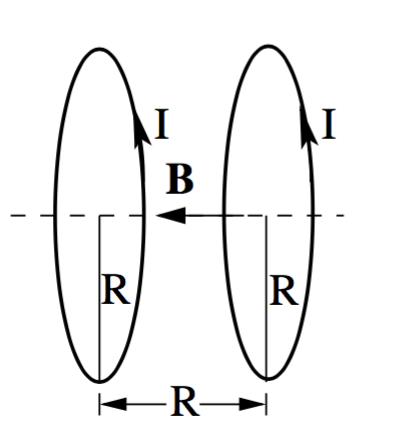
\includegraphics[height=5cm]{Helmholtz.png}
    \caption{Skizze einer Helmholtzspule \cite{skript}}
    \label{fig:helm}
  \end{figure}

  \noindent Hierdurch ergibt sich im Zentrum wieder ein homogenes
  Magnetfeld, welches durch die Überlagerung der beiden einzelnen Felder durch Gleichung
  \ref{eqn:Biot2} zu
  \begin{equation}
    B(x)= \frac{\mu_0 \cdot I \cdot R^2}{(R^2 + x^2)^{3/2}}
    \label{eqn:Helmholtz}
  \end{equation}
  ergibt, wobei der Gradient entlang der Achse durch die Formel
  \begin{equation}
    \frac{dB}{dx} = -3\mu_0 \cdot I \cdot R^2 \frac{x}{(R^2+x^2)^(5/2)}
    \label{eqn:gradient}
  \end{equation}
bilden lässt. \\

\noindent In einem ferromagnetischen Material gibt es permanente magnetische Momente,
welche sich in kleinen Bereichen, den sogenannten Weiß´schen Bezirken, gegenseitig
beeinflussen und sich somit parallel zueinander ausrichten. Wird hier ein äußeres
Magnetfeld angelegt, richten sich die zunächst zufällig verteilten Bereiche nach und
nach entlang
der Magnetfeldlinien aus, bis alle Weiß´schen Bezirke in Richtung des Magnetfelds liegen,
das ursprüngliche Feld wird somit verstärkt.
In solchen Materialien ist die relative Permeabilität $\mu_r $ sehr hoch und unterliegt zudem
nicht mehr der linearen Beziehung aus Gleichung \ref{eqn:B1}, sondern ergibt sich als
Funktion der magnetischen Feldstärke H, wobei sie in Größenordungen von
$10^2$ bis $10^7$ liegt. Dazu verwendet man die differentielle Permeabilität
$\mu_{diff}$ mit
\begin{equation}
  \mu_{diff} = \frac{1}{\mu_0}\frac{dB}{dH}
  \label{eqn:mur}
\end{equation}
\noindent Dadurch ergibt sich die
sogenannte Hysterese-Kurve, die in \ref{fig:hysterese}
dargstellt ist.
\begin{figure}[H]
  \centering
  \includegraphics[height=5cm]{hysterese.png}
  \caption{Skizze einer Hysteresekurve \cite{skript}}
  \label{fig:hysterese}
\end{figure}
\noindent Dadurch, dass nach einer Magentisierung auch ohne äußeres Magnetfeld
noch eine Restmagnetisierung bestehen bleibt hängt der Verlauf von der vorherigen Geschichte
des Materials ab und ist somit nicht eindeutig.
\\
\noindent Ist die Verteilung der Weiß´schen Bezirke zunächst zufällig verteilt,
steigt die Magnetisierung asymptotisch gegen einen Sättigungswert $B_s$, bei welchem dann alle
Weiß´schen Bezirke ausgerichtet sind. Der Verlauf dieses Prozesses wird Neukurve
(in der Abbildung: Verlauf (1)) genannt. Wird das äußere Magnetfeld dann abgeschaltet,
bleibt die bereits erwähnte Restmagnetisieung, welche als Remanenz bezeichnet wird.
Um diese zu entfernen, muss ein entgegengerichtetes Magnetfeld angelegt werden, was
als Koerzitivkraft $H_c $ bezeichnet wird. Wird das Gegenfeld weiter erhöht, läuft die
Magnetisierung dann asymptotisch gegen den negativen Wert der Remanenz $-B_s$ (Verlauf(2)).
Durch ein erneut positives Feld ergibt sich nun wieder ein Verlauf (3), welcher punktsymmetrisch
zu Verlauf (2) ist und erneut gegen $B_s$ strebt.
Die breite und die Eigenschaften der Hysterese-Kurve hängen hierbei von den
Eigenschaften des zu untersuchenden Materials ab.\\
\noindent
Wird ein ferromagnetisches Material in eine Spule gebracht, ergibt sich der dadurch
erhöhte magnetische Fluss zu
\begin{equation}
  \vec{B}= \mu_0 (\vec{H}+\vec{M}) = \mu_0 (\vec{H_0}+ \vec{H_r} +\vec{M})
\end{equation}
wobei durch $\vec{H_r}$ auch Randeffekte berücksichtigt werden. Dieser Term fällt
bei Toroid-Spulen jedoch weg, sodass hier die Relation $\vec(H) = \vec{H_0} =
\vec{B}\/ \mu_o $ gilt.
